\begin{figure}[htbp]
\centering
\shorthandoff{<>}
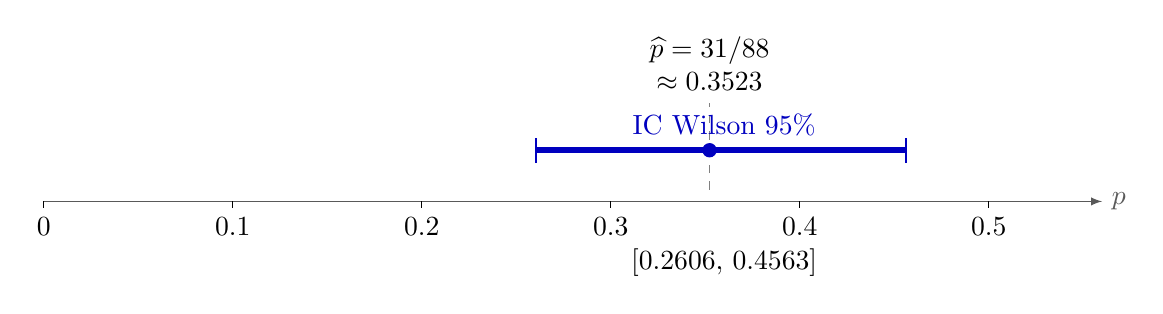
\begin{tikzpicture}[x=24cm,y=1cm,font=\normalsize,>=latex]
  \draw[->,black!65] (0,0) -- (0.56,0) node[right] {$p$};
  \foreach \x in {0,0.1,0.2,0.3,0.4,0.5}{\draw (\x,0)--(\x,-0.08) node[below] {$\x$};}
  \draw[gray,dashed] (0.35227,0.15) -- (0.35227,1.25);
  \node[above,align=center] at (0.35227,1.28) {$\widehat p=31/88$\\$\approx0.3523$};
  \draw[blue!75!black,line width=2pt] (0.26056,0.65) -- (0.45634,0.65);
  \draw[blue!75!black,thick] (0.26056,0.49)--(0.26056,0.81);
  \draw[blue!75!black,thick] (0.45634,0.49)--(0.45634,0.81);
  \fill[blue!75!black] (0.35227,0.65) circle (2.6pt);
  \node[above,blue!75!black] at (0.36,0.70) {IC Wilson 95\%};
  \node[below,align=center] at (0.36,-0.48) {$[0.2606,\,0.4563]$};
\end{tikzpicture}
\shorthandon{<>}
\caption{Intervalo de confianza de Wilson del 95\% para la proporción poblacional. La línea punteada marca la proporción observada y los extremos azules, los límites de confianza; el eje horizontal representa la proporción de binarias eclipsantes en la población.}
\label{fig:intervalo-binomial}
\end{figure}